\section{Scheduling}\label{scheduling}

\subsection{Rappel}\label{rappel}

Les SE tel que Linux supporte d'avoir un grand nombre de thread (parfois
sur des mono-processeurs). On doit donc partager. On crée l'illusion de
continuité.

\subsection{Mécanisme \& Politique}\label{muxe9canisme-politique}

\begin{itemize}
\tightlist
\item
  \textbf{Mécanisme:} (\emph{ex:} changement de contexte (sauvegarde et
  restauration)) cela permet d'\textbf{acter des décisions de placement
  de threads sur les processus}.
\item
  \textbf{Politique} (\emph{ex:} scheduler ) cela permet de
  \textbf{prendre des des décisions de placement} (ou va chaque
  threads).
\end{itemize}

Donc on peut avoir plusieurs politiques possibles sur la base du même
mécanisme.

\subsubsection{Exécution des Threads}\label{exuxe9cution-des-threads}

\begin{figure}
\centering
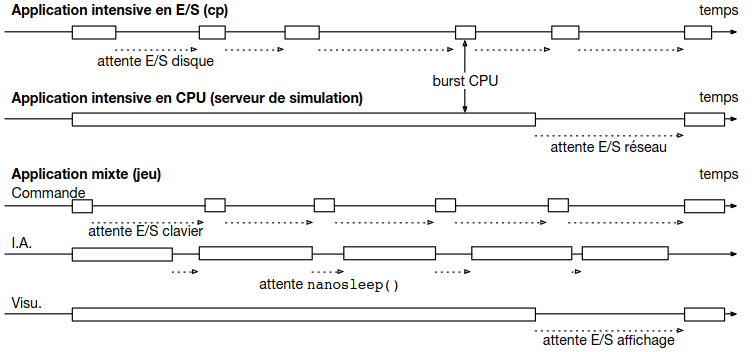
\includegraphics{image-28.png}
\caption{Alt text}
\end{figure}

On a une alternance entre:

\begin{enumerate}
\def\labelenumi{\arabic{enumi}.}
\tightlist
\item
  \textbf{Burst CPU}
\item
  \textbf{Opération bloquante}
\end{enumerate}

Sur le schéma ci-dessus, on voit la durée de différent burst CPU et les
moments d'attente.

\begin{figure}
\centering
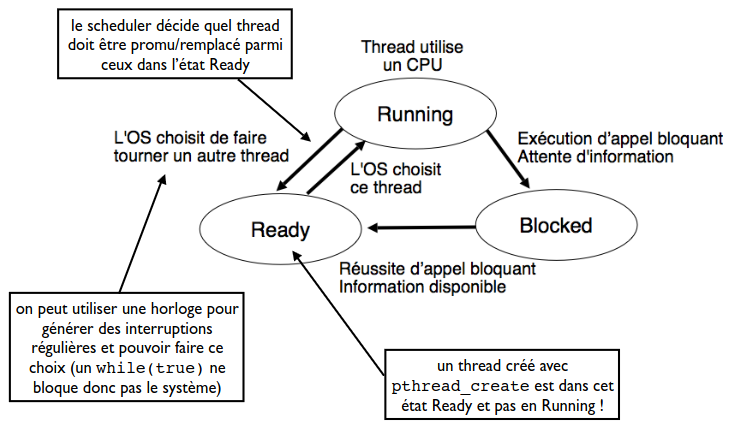
\includegraphics{image-29.png}
\caption{une image vaut mieux que mille mots}
\end{figure}

\subsubsection{Évolution de l'État d'un
Thread}\label{uxe9volution-de-luxe9tat-dun-thread}

\paragraph{\texorpdfstring{Passage de \emph{Running} à
\emph{Blocked}}{Passage de Running à Blocked}}\label{passage-de-running-uxe0-blocked}

\begin{itemize}
\tightlist
\item
  Appel système \emph{bloquant} (ex: \emph{pthread\_mutex\_lock(3
  posix)}, \emph{read(2)}, \emph{sem\_wait(3posix)})
\end{itemize}

Les threads en état Blocked associés à une structure de donnée jouant le
rôle d'une \emph{salle d'attente}.

\begin{itemize}
\tightlist
\item
  \emph{Thread Unique}: attente de la fin d'une entrée/sortie demandée
  par ce thread
\item
  \emph{Plusieurs Threads}: attente sur une ressource partagée (type
  \emph{sémaphore} / \emph{mutex})
\end{itemize}

\begin{figure}
\centering
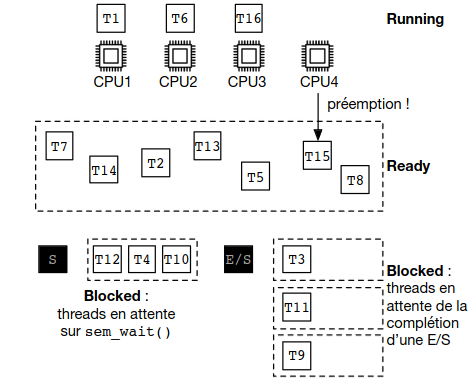
\includegraphics{image-30.png}
\caption{Alt text}
\end{figure}

On a aucune garantie sur l'ordre de réveil de thread

\paragraph{\texorpdfstring{Passage de \emph{Running} à
\emph{Ready}}{Passage de Running à Ready}}\label{passage-de-running-uxe0-ready}

On va sé prémunir des programmes qui sont \emph{infiniment} en mode
\emph{ready}.

Le SE va faire des interruptions périodiques générées par une horloge.
Ensuite, le SE peut décider de \textbf{ne pas restaurer} le thread
Running. On appelle cela la \textbf{préemption}.

\paragraph{\texorpdfstring{Passage de \emph{Ready} à
\emph{Running}}{Passage de Ready à Running}}\label{passage-de-ready-uxe0-running}

Le \emph{Scheduler} a décidé de restaurer l'état de ce thread sur le
processeur.

\subsection{Scheduler}\label{scheduler}

Le \emph{Scheduler} fait une \textbf{politique d'ordonnancement}. Ce
dernier prend des décisions à deux occasions:

\begin{enumerate}
\def\labelenumi{\arabic{enumi}.}
\tightlist
\item
  \textbf{Processeur disponible}: à la fin d'un CPU Burst.
\item
  \textbf{Interruption périodique}: peut arriver pendant un CPU Burst.
\end{enumerate}

Dans le cas 2. le scheduler est donc \textbf{préemptif}.

\paragraph{Scheduler Universel}\label{scheduler-universel}

Il n'y a pas de scheduler parfait.

\subsubsection{Objectifs}\label{objectifs}

On doit faire un compromis entre différents objectifs:

\begin{itemize}
\tightlist
\item
  \textbf{Objectifs Systèmes:}

  \begin{itemize}
  \tightlist
  \item
    Maximiser l'utilisation processeur
  \item
    Maximiser le débit applicatif
  \end{itemize}
\item
  \textbf{Objectifs pour chaque Application:}

  \begin{itemize}
  \tightlist
  \item
    Minimiser le temps d'exécution total (pas de sens pour application
    interactive)
  \item
    Minimiser le temps d'attente (entre \emph{Ready} vers
    \emph{Running})
  \item
    Minimiser le temps de réponse (entre \emph{Ready} vers
    \emph{Blocked})
  \item
    Équité des métriques
  \end{itemize}
\end{itemize}

\subsubsection{Scheduler FCFS}\label{scheduler-fcfs}

\textbf{First-Come First-Serve}. Le scheduler est donc non préemptif car
un thread Running complète tout son burst CPU.

Ainsi avec 4 threads avec un temps d'exécution respectif de 5,4,2 et 7
secondes. On peut avoir une attente moyenne de 7 ou 5 secondes.

Ce n'est pas optimal pour des burst CPU plus court qui sont coincés
derrière des burst plus long.

\subsubsection{Scheduler SJF}\label{scheduler-sjf}

Choisit le thread Ready avec le burst CPU le plus court. Toujours non
préemptif. Et va trouver le temps le plus court (dans notre exemple
d'au-dessus, le temps d'attente moyen le plus court est 4.25 secondes).

Mais connaître le temps d'arrêt d'un thread revient à transgresser le
\textbf{problème de l'arrêt}.

On peut néanmoins prédire les prochains burst basés sur les précédents.
On va donc utiliser des moyennes pondérées comme estimation.

\begin{figure}
\centering
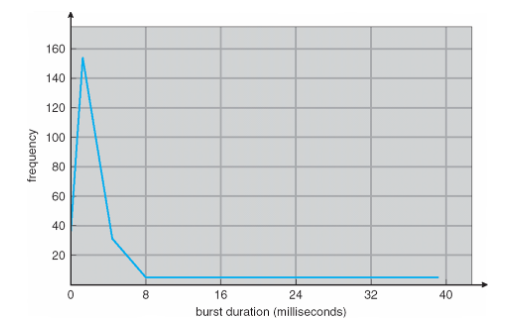
\includegraphics{image-31.png}
\caption{Burst typique}
\end{figure}

Avec ce type d'organisation, les bursts les plus longs risquent de
rester bloquer derrière les plus courts de manière indéfinie.

\subsubsection{Scheduler Préemptif RR}\label{scheduler-pruxe9emptif-rr}

On peut libérer le processeur à chaque tick de l'horloge système. C'est
un équivalent de \emph{Round-Robin} (ruban rond).

\begin{figure}
\centering
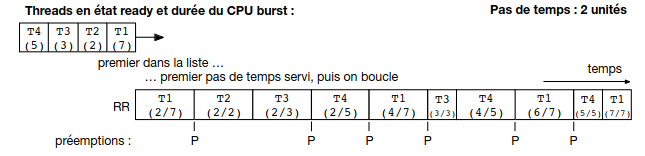
\includegraphics{image-32.png}
\caption{Alt text}
\end{figure}

\begin{itemize}
\tightlist
\item
  ✅ Ainsi, on a un temps d'attente moyen assez court.
\item
  ❌ Pas de relation directe entre \emph{attente} et \emph{temps de
  réponse}
\item
  ❌ Beaucoup de changement de contexte
\item
  ❌ Pas de distinction entre threads avec bursts courts et longs
\end{itemize}

\paragraph{Fréquence d'horloge}\label{fruxe9quence-dhorloge}

Au + la fréquence est haute, au - temps d'attente des threads
\textbf{mais} + de consommation d'énergie et - d'utilisation utile du
CPU

\begin{itemize}
\tightlist
\item
  1990: 100 Hz
\item
  2000: 1 kHz
\item
  2010+: fréquence adaptive (base clock et boost clock). Pas de réveil
  d'un processeur en veille si pas de thread \emph{Ready}. Pas
  d'interruption si un seul thread \emph{Running} et pas de
  \emph{Ready}.
\end{itemize}

\subsubsection{Scheduler à Priorité}\label{scheduler-uxe0-priorituxe9}

Pas la même priorité pour différentes applications: \emph{daemon} vs
\emph{application utilisée par l'utilisateur à l'instant t}.

Pareil pour les threads, certains vont demander de la réactivité et des
ressources et d'autres non.

On va exécuter le thread avec la plus haute priorité d'abord. On
maintient une liste circulaire. Il faut faire attention au problème de
famine

\paragraph{Problème de Famine}\label{probluxe8me-de-famine}

On utilise des priorités adaptatives (\emph{basse} et \emph{courante}).

Au départ: priorité courante = priorité de base

À chaque exécution d'un burst CPU, la priorité courante diminue. On
réalise un nouveau cycle quand tous les threads ont une priorité
courante = 0.

\paragraph{Tout Combiner}\label{tout-combiner}

On combine les principes de priorité + préemption.

\begin{itemize}
\tightlist
\item
  Thread passe Running: on lui alloue un temps d'exécution maximale =
  \textbf{quantum} (longueur du quantum = multiple de la période de
  l'horloge système).
\item
  Thread termine dans les temps sinon préemption.
\item
  Utilisation de priorités fixes et courantes (courante diminue à chaque
  burst CPU).
\end{itemize}

\begin{figure}
\centering
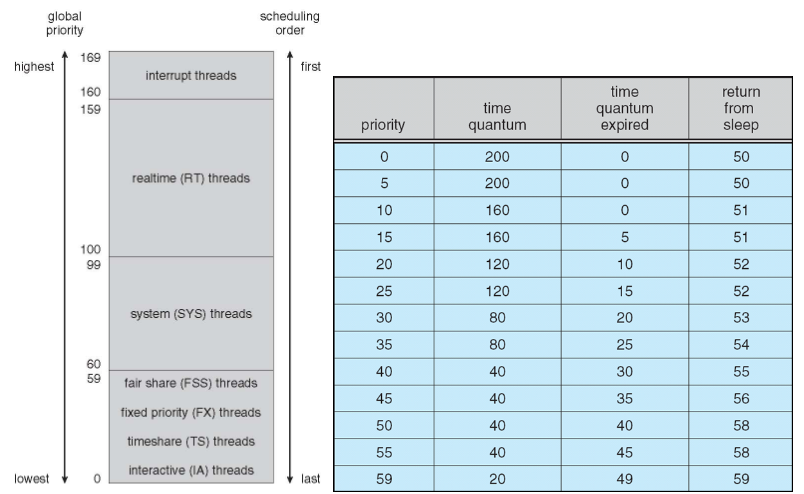
\includegraphics{image-33.png}
\caption{Alt text}
\end{figure}

\paragraph{Synchronisation des
Threads}\label{synchronisation-des-threads}

Il vaut mieux laisser un thread de priorité basse finir sa section
critique plutôt que de la préempter.

\begin{itemize}
\tightlist
\item
  \textbf{\emph{Priority ceiling:}}
  \texttt{pthread\_mutexattr\_setprioceiling()}

  \begin{itemize}
  \tightlist
  \item
    Associe un mutex de priorité donné au thread le temps de sa SC. Fixé
    au max des priorités des threads accédant au mutex.
  \item
    Évite la préemption par le thread de priorité plus élevée. Risque
    d'interférence avec les autres threads haute priorité dy système car
    fait systématiquement.
  \end{itemize}
\item
  \textbf{\emph{Priority inheritance:}}

  \begin{itemize}
  \tightlist
  \item
    La priorité du thread avec un mutex est fixée au max de celle des
    threads en attente sur ce mutex.
  \item
    N'évite pas la première préemption mais booste la priorité d'un
    thread de priorité faible dans le cas général.
  \end{itemize}
\end{itemize}

\paragraph{Priorité des Processus}\label{priorituxe9-des-processus}

Par défaut, les threads d'un processus héritent de la priorité du
premier thread du processus. Dépend donc de l'environnement d'exécution.

Si on est pas \texttt{root}, on ne peut pas demander des priorités plus
élevés mais \emph{seulement} plus faibles.

On fait cela via l'utilitaire \texttt{nice(1)} ou la fonction
\texttt{nice(2)}.

\begin{itemize}
\tightlist
\item
  \(>0\): priorité plus faible (jusqu'à 20)
\item
  \(<0\); priorité plus élevé (jusqu'à -19)
\end{itemize}

\subsection{Conclusion}\label{conclusion}

À la base d'un même mécanisme de changement de contexte, plusieurs
politiques différentes possibles

\begin{itemize}
\tightlist
\item
  On peut utiliser de l'apprentissage automatique pour améliorer les
  paramètre d'un scheduler
\end{itemize}

Dans Linux, les priorités sont dynamiques et prise en compte des threads
\emph{interactifs}/\emph{intensifs} en CPU.

\begin{itemize}
\tightlist
\item
  Le noyau supporte de nombreux scheduler différents
\item
  Chaque scheduler peut être paramétré
\item
  Critique pour la bonne performance et l'efficacité énergétique
\end{itemize}
